\documentclass{article}
\usepackage{graphicx}
\usepackage{amsmath} 
\usepackage{amssymb}
\usepackage{graphicx}

\title{18786 HW3 Report}
\author{YIZHEN XU}
\date{February 2026}

\begin{document}

\maketitle

\section{Position Embeddings Exploration}

\subsection*{Question 1: Permuting the Input}

\begin{enumerate}
    \item[i.] Proof of Permutation Equivariance \\
    Suppose we have a permutation matrix $P \in \mathbb{R}^{T \times T}$ and the permuted input $X_{\text{perm}} = PX$. The Query, Key, and Value matrices are transformed as:
    \begin{equation}
        Q_p = PXW^Q = PQ, \quad K_p = PXW^K = PK, \quad V_p = PXW^V = PV
    \end{equation}
    The attention score matrix $A_p$ for the permuted input is:
    \begin{equation}
        A_p = \frac{Q_p K_p^\top}{\sqrt{d_k}} = \frac{(PQ)(PK)^\top}{\sqrt{d_k}} = P \left( \frac{QK^\top}{\sqrt{d_k}} \right) P^\top = PAP^\top
    \end{equation}
    Using the given property $\text{softmax}(PAP^\top) = P \text{softmax}(A) P^\top$:
    \begin{equation}
        \text{Attn}_{p} = \text{softmax}(A_p) = P \text{softmax}(A) P^\top
    \end{equation}
    The final output $Z_{\text{perm}}$ is obtained by:
    \begin{equation}
        Z_{\text{perm}} = \text{Attn}_{p} V_p = (P \text{softmax}(A) P^\top)(PV)
    \end{equation}
    Since $P^\top P = I$ for any permutation matrix:
    \begin{equation}
        Z_{\text{perm}} = P \text{softmax}(A) I V = P (\text{softmax}(A)V) = PZ
    \end{equation}
    This demonstrates that Shuffling the input leads to an identically shuffled output.

    \item[ii.] \textbf{Implications for NLP} \\
    This result proves that the standard Self-Attention mechanism is permutation equivariant, meaning it treats the input as a "bag of words" rather than a sequence. In natural language, word order is fundamental to meaning. Without positional information, the model cannot distinguish between different permutations of the same tokens, which is why positional encodings are strictly required to break this symmetry.
\end{enumerate}

\subsection*{Question 2: Position Embeddings}

The position embeddings $\Phi \in \mathbb{R}^{T \times d}$ are defined as:
\begin{equation}
    \Phi_{(t, 2i)} = \sin(t/10000^{2i/d}), \quad \Phi_{(t, 2i+1)} = \cos(t/10000^{2i/d})
\end{equation}
The input becomes $X_{\text{pos}} = X + \Phi$.

\begin{enumerate}
    \item[i.] Effectiveness \\
    Yes, position embeddings resolve the issue identified in part (a). By adding $\Phi$, the input for each token becomes dependent on its absolute position $t$. Consequently, $X_{\text{pos}}$ no longer satisfies the permutation property $P(X+\Phi) \neq PX + \Phi$ (unless $P=I$), which breaks the symmetry and allows the model to utilize structural information.

    \item[ii.] Uniqueness of Embeddings \\
    No, the position embeddings for two different tokens cannot be the same. Each position $t$ results in a unique combination of sine and cosine waves of different frequencies across the dimension $d$. Since the period of the functions increases with $i$, the vector $\Phi_t$ effectively acts as a unique signature for each time step $t \in [0, T-1]$, ensuring that no two positions share the same encoding within reasonable sequence lengths.
\end{enumerate}

\section{Pretrained Transformer models and knowledge access}

\subsection*{(d) Make predictions (without pretraining)}
\begin{itemize}
    \item \textbf{None-pretrain Model:} Testing the model directly without any pretraining yielded an accuracy of \textbf{0.8\%} on the validation set. 
    \item \textbf{London Baseline:} By implementing a simple baseline that predicts ``London'' for every query using \texttt{london\_baseline.py}, we achieved an accuracy of \textbf{5\%} on the validation set. 
\end{itemize}

\subsection*{(e) Define a span corruption function for pretraining}
\begin{figure}[h]
    \centering
    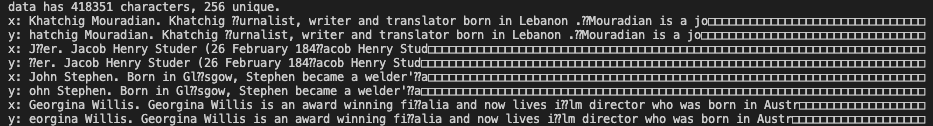
\includegraphics[width=1.0\textwidth]{q2e.png}
    \caption{Output of charcorruption}
    \label{fig:my_image}
\end{figure}

\subsection*{(f) Pretrain, finetune, and make predictions}
\begin{itemize}
    \item Accuracy on the dev set: 24.6\%. The jump in accuracy from the London baseline (5\%) and the randomly initialized model (0.8\%) to 24.6\% demonstrates the effectiveness of pretraining.
\end{itemize}

\subsection*{ (g) Write and try out a different kind of position embeddings}

\begin{enumerate}
    \item[i.] RoPE Rotation Interpretation \\
    To show that the elements of the vector in Equation 1 can be obtained from Equation 2, we expand both expressions. In Equation 1, the first two elements resulting from the first $2 \times 2$ rotation block are:
    \begin{equation}
        y_t^{(1)} = x_t^{(1)} \cos t\theta_1 - x_t^{(2)} \sin t\theta_1, \quad y_t^{(2)} = x_t^{(1)} \sin t\theta_1 + x_t^{(2)} \cos t\theta_1
    \end{equation}
    In Equation 2, we perform element-wise complex multiplication. The first component is:
    \begin{equation}
        (\cos t\theta_1 + i \sin t\theta_1) \cdot (x_t^{(1)} + i x_t^{(2)})
    \end{equation}
    Expanding this product using the distributive property $(ac - bd) + i(ad + bc)$, we obtain:
    \begin{equation}
        (x_t^{(1)} \cos t\theta_1 - x_t^{(2)} \sin t\theta_1) + i (x_t^{(1)} \sin t\theta_1 + x_t^{(2)} \cos t\theta_1)
    \end{equation}
    By inspection, the real part of the complex product matches the first element of Equation 1, and the imaginary part matches the second element. This relationship holds for all $d/2$ blocks. Therefore, Equation 1 can be retrieved by reshaping the complex vector from Equation 2 such that the real and imaginary components are interleaved as consecutive elements.

    \item[ii.] Relative Embeddings \\
    To show that the dot product of RoPE embeddings depends only on the relative position $t_1 - t_2$, we use the complex representation where $RoPE(z, t) = z e^{it\theta}$. Using the provided hint for the dot product of complex numbers $\langle z_1, z_2 \rangle = Re(\bar{z}_1 z_2)$, we have:
    \begin{equation}
        \langle RoPE(z_1, t_1), RoPE(z_2, t_2) \rangle = Re\left( \overline{z_1 e^{it_1\theta}} \cdot (z_2 e^{it_2\theta}) \right)
    \end{equation}
    Applying the property of complex conjugates $\overline{ab} = \bar{a}\bar{b}$ and $\overline{e^{i\phi}} = e^{-i\phi}$:
    \begin{equation}
        Re\left( \bar{z}_1 e^{-it_1\theta} z_2 e^{it_2\theta} \right) = Re\left( \bar{z}_1 z_2 e^{i(t_2 - t_1)\theta} \right)
    \end{equation}
    Now, consider the right-hand side of the required identity $\langle RoPE(z_1, t_1 - t_2), RoPE(z_2, 0) \rangle$:
    \begin{equation}
        Re\left( \overline{z_1 e^{i(t_1 - t_2)\theta}} \cdot z_2 \right) = Re\left( \bar{z}_1 e^{-i(t_1 - t_2)\theta} z_2 \right) = Re\left( \bar{z}_1 z_2 e^{i(t_2 - t_1)\theta} \right)
    \end{equation}
    Since both sides expand to the same expression, we have shown that $\langle RoPE(z_1, t_1), RoPE(z_2, t_2) \rangle = \langle RoPE(z_1, t_1 - t_2), RoPE(z_2, 0) \rangle$. This proves that the self-attention mechanism using RoPE is sensitive to the relative distance between tokens, which is a desirable property for modeling sequential dependencies in text.

    \item[iii.] Train and evaluate with RoPE \\
    Accuracy on the development set: 38.0\% \\
    Analysis: The significant increase in accuracy to 38.0\%, compared to the 24.6\% achieved with absolute position embeddings, demonstrates that RoPE is more effective at capturing the relative spatial relationships between tokens. By encoding positional information as rotations in a complex vector space, the model maintains better sensitivity to the relative distance between names and their corresponding birthplaces, leading to superior knowledge retrieval performance.
    
\end{enumerate}

\section{Considerations in pretrained knowledge}
\begin{enumerate}
    \item[a.] Pretrained vs Non-pretrained Performance \\
    The pretrained model achieved higher accuracy because it learned latent factual associations and general linguistic patterns from the large-scale corpus (wiki.txt) during its pretraining phase. This allows the model to retrieve internal knowledge of entity relationships, such as names and locations, which is entirely absent in the randomly initialized weights of the non-pretrained model.

    \item[b.] Implications of Indistinguishable Hallucinations \\
    \begin{itemize}
        \item Concern 1: Misplaced Trust and Safety. Since the model produces incorrect facts (hallucinations) with the same linguistic confidence as correct ones, users may rely on false information for critical decision-making. Example: A researcher citing a fabricated birthplace of a historical figure provided by the model.
        \item Concern 2: Difficulty in Debugging and Filtering. Without a mechanism to distinguish retrieval from generation, it is impossible for developers to implement reliable filters to catch errors. Example: A medical assistant providing a fake drug contraindication that looks identical in format to a real one.
    \end{itemize}

    \item[c.] Strategy for Unseen Entities and Potential Concerns \\
    For a name never encountered during pretraining or fine-tuning, the model may resort to a strategy based on statistical heuristics or stereotypes associated with the name's morphology or linguistic origin. For instance, it might predict a German city for a name that sounds Germanic. This is highly problematic because it introduces systemic bias and reinforces cultural stereotypes, leading to unfair or discriminatory outputs in user-facing applications.
\end{enumerate}

\section{Modern LLM and Prompt Sensitivity}

\begin{enumerate}
    \item[a.] Impact of Prompt Reformatting \\
    Changing the prompt format to "What is the birthplace of ...?" resulted in an accuracy of 15.8\%. This gap occurs because the model overfits to the specific syntactic structure used during finetuning. Even with identical semantics, the model fails to trigger the same knowledge retrieval mechanism when the prompt structure deviates from the training template.

    \item[b.] Inference with Instruction-Tuned LLMs \\
    The reported accuracy was 0\% because instruction-tuned models are optimized for conversational fluency. Instead of providing the exact single-word label, the model generates complete sentences. Since the evaluation script relies on strict string matching against the ground truth, any additional conversational verbiage results in a technical accuracy of zero.

    \item[c.] Optimization through Prompt Engineering and Output Parsing \\
To address the zero accuracy observed in instruction-tuned models, several strategic modifications were implemented to align the model's outputs with the strict evaluation format. 

\begin{itemize}
    \item Reasoning Extraction: Added logic to detect the closing \textit{</think>} tag, discarding internal chain-of-thought content and preserving only the final answer.
    \item Context Window Adjustment: Increased \textit{max\_new\_tokens} to 512 to ensure the model has sufficient budget to complete its reasoning and reach the conclusion.
    \item Constraint Prompting: Updated the system prompt with explicit instructions to "Answer with the city or country name only," discouraging conversational filler.
    \item Post-processing Refinement: Implemented cleaning logic to remove common sentence prefixes (e.g., "The answer is"), strip country suffixes via comma splitting, and remove terminal punctuation.
\end{itemize}

The obtained accuracies are as follows:
\begin{itemize}
    \item Original template ("Where was ... born?"): 11.2\%
    \item Modified template ("What is the birthplace of ...?"): 11.0\%
\end{itemize}
\end{enumerate}



\end{document}